\section{Regularization}

\subsection{}

\begin{frame}
    \frametitle{Underfitting and overfitting}

    \begin{alertblock}{Danger!}
        Neural networks are hard to fit, and real-life data are noisy.
        \emph{Underfitting} and \emph{overfitting} are your two biggest obstacles.
    \end{alertblock}
    \vspace{1ex}

    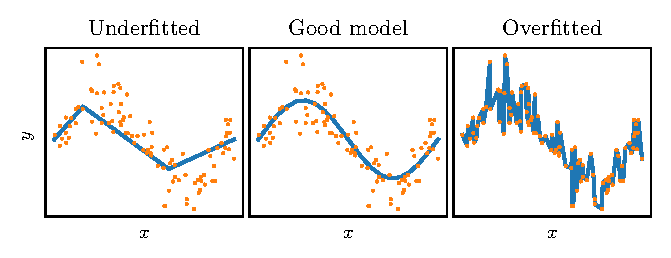
\includegraphics{under_over_train}
    \pause

    \begin{itemize}
        \item Underfitting: didn't train enough for the model to capture the underlying behavior
        \item Overfitting: training so good that neural network memorizes the data, including underlying noise
        \begin{itemize}
            \item Recall: with enough parameters, neural networks learn anything
        \end{itemize}
    \end{itemize}
\end{frame}

\begin{frame}
    \frametitle{Train, validate, test}

    Usual trick: split data into disjoint \textcolor{blue}{training} and \textcolor{Green4}{testing} sets
    \begin{itemize}
        \item Anywhere from 95/5 to 75/25 split is common
        \item Train \emph{only} on the \textcolor{blue}{training set}
        \item Periodically check loss of NN on \textcolor{Green4}{test set}
        \begin{itemize}
            \item Optimizer never sees test set: test set is honest check on NN fidelity
        \end{itemize}
    \end{itemize}
    \pause

    More advanced: split into disjoint \textcolor{blue}{training}, \textcolor{orange}{validation}, and \textcolor{Green4}{testing} set
    \begin{itemize}
        \item Aside on terminology
        \begin{itemize}
            \item Weights \& biases are \alert{parameters}---iteratively improved
            \item Design choices (\# layers, \# neurons, optimizer, \# epochs, etc.) are \alert{hyperparameters}---selected by ML designer
        \end{itemize}
        \item Select different sets of hyperparameters; for each:
        \begin{itemize}
            \item Train only on \textcolor{blue}{training set}, as before
            \item Compute validation loss on \textcolor{orange}{validation set}
        \end{itemize}
        \item Pick hyperparameters with lowest validation loss
        \item Then re-evaluate loss on \textcolor{Green4}{test data}
        \begin{itemize}
            \item Helps remove effects of variance on validation loss
        \end{itemize}
    \end{itemize}
\end{frame}

\begin{frame}
    \frametitle{Training loss vs.~test loss}
    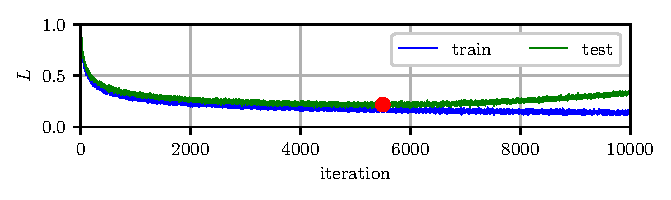
\includegraphics{loss}

    General pattern
    \begin{itemize}
        \item Modulo minor stochastic fluctuations, training loss should monotonically decrease: NN gets better at learning data
        \item Test loss usually at least slightly larger than training loss
        \begin{itemize}
            \item Because optimizer minimizes training loss but never sees test data
        \end{itemize}
        \item At some point, test loss increases: NN overfits to training data
        \item \alert{Early stopping}: use NN with minimum test loss
    \end{itemize}
\end{frame}

\begin{frame}
    \frametitle{Regularization techniques}

    \begin{block}{}
        Regularization: modifications that reduce generalization error
    \end{block}

    \begin{itemize}
        \item Early stopping
        \item Weight penalization
        \item Dropout
        \item Bagging
        \item Boosting
    \end{itemize}
\end{frame}

% Dropout
% Noise
% Weight clipping
% Weight penalty

%%% Local Variables:
%%% mode: latex
%%% TeX-master: "../nn"
%%% End:
